\graphicspath{{testing_and_validation/fig/}}

\chapter{Testing \& Validation}

The testing and validation process was structured to systematically verify the functionality of the impedance analyser, progressing from subsystem verification to complete system integration and finally calibration and validation with \acp{IDE} and lab tests.

% Testing began with fundamental verification of the assembled PCB, followed by individual subsystem characterisation. Once subsystem functionality was established, the complete analogue frontend was tested as an integrated system. Finally, the device was calibrated against the PalmSens4 impedance analyser and validated using biosensors with buffer solutions.

\section{PCB Testing Methodology and Results}

The assembled PCB was visually inspected, and continuity testing confirmed no obvious short circuits or discontinuities. The ESP32's onboard battery charging circuit and regulator was confirmed to supply a stable 3.3 V rail to all digital and analogue components with enough current to avoid brownouts. The virtual ground reference circuit was measured at exactly 1.650 V. The TPS61072 boost converter successfully provided a stable 5 V supply for the LTC1069 anti-aliasing filter.

Next, each subsystem was tested individually whilst other subsystems remained disconnected. This approach allowed for precise characterisation of each stage's performance and simplified fault diagnosis.

\subsection{Excitation Stage} 
The excitation stage was tested using a signal generator providing a 3 Vpp input signal and an oscilloscope to measure the attenuated output. Unfortunately, the LTC1069 anti-aliasing filter was found to be dead-on-arrival. Given the significant lead times for component procurement and project time constraints, it was not feasible to order a replacement. The filter would have improved performance at very low frequencies, but was not a critical part of the system and therefore the excitation stage was tested without it. Whilst this introduces higher-frequency components from the DAC's stairstepping, the synchronisation of DAC generation and ADC sampling and FFT frequency extraction helps to minimise the impact on measurements.
The attenuation stage was characterised across the full frequency range from 1 Hz to 100 kHz. The resulting signal was measured at $\approx$10.33 mVpp, giving a 290 V/V attenuation, with a flat frequency response. This is close to the designed 10 mVpp and well within the ideal range for biosensing applications and our voltage measurement stage.

% Figure \ref{fig:excitation_freq_response} shows the frequency response, which exhibits a flat gain and phase across the measurement range.
% \todo{Move fig to appendix}
% \begin{figure}[H]
%     \centering
%     % \includegraphics[width=0.8\textwidth]{ExcitationFreqResponse.png}
%     \caption{Excitation Stage Frequency Response}
%     \label{fig:excitation_freq_response}
% \end{figure}

\subsection{Voltage Measurement Stage} 
For the voltage measurement stage, both the INA331 instrumentation amplifier and TLV9061 gain stage were tested separately. The INA331 was tested using a 200mV input signal to minimise noise from the signal generator. It performed as expected, with no measurable gain roll-off at 100 kHz and a phase shift of -5\textdegree, which is close to the expected -4.6\textdegree\ based on simulations.

The TLV9061 stage was similairly tested using a 150mV input signal to avoid clipping on the output. It performed well, exhibiting a less than 0.2 dB gain roll-off and -8.7\textdegree\ phase shift at 100 kHz compared to the expected -3.4\textdegree. The larger-than-expected phase shift can be attributed to tolerances in the op-amp's gain-bandwidth product.

Overall, the voltage measurement stage's performance closely matched expectations, with the phase offsets remaining well within acceptable limits for accurate impedance measurements if properly calibrated for.

% \todo{Insert Table wat cutoff en 100kHz summarise vir elke afdeling en dan langs dit grafiek wat responses van elke substage wyse op eenm grafiek}
While the applied voltage is roughly known, the current varies significantly based on the impedance. Therefore, the current measurement stage was the most critical to verify.


\subsection{Current Measurement Stage} 
The current measurement stage required the most extensive testing due to its complexity and switchable gain configurations.

The TIA was characterised by applying known voltages across resistors of known values, allowing the input current to be calculated. The TIA output voltage was then measured to determine the transimpedance gain across the full frequency range. The resistor values were measured using a standard multimeter (rather than a Kelvin sense connection) and the resistors' parasitic inductance and capacitance were ignored. However, this characterisation served primarily for functional validation, as final calibration would be performed against the PalmSens4.

At $R_f = 37.5~\Omega$, the TIA exhibited a gain of 37.73 V/V with a phase shift of -4.4\textdegree\ and gain reduction of 0.74 dB at 100 kHz. At the larger feedback resistor value of $R_f = 7.5~k\Omega$, the gain averaged at 7427 V/V. Interestingly, both phase shift and gain reduction  at 100 kHz were less pronounced with the higher feedback value at -3.5\textdegree\ and \textless 0.1 dB respectively. This is possibly due to slight peaking.

Stability was verified by connecting a simplified Randles equivalent circuit with a constant capacitance of \SI{1.47}{\micro F} and resistance of $12~\Omega$, approximating the expected biosensor characteristics (Table \ref{tab:stability_params}). A 10 mVpp signal was applied to the equivalent circuit and swept from 1 Hz to 30 MHz while monitoring the TIA output for oscillations, ringing, or excessive peaking in the frequency response. No instability was observed, confirming the theoretical analysis in Section \ref{subsec:design_cur}.

The PGA113 was measured at each gain setting from 1 V/V to 200 V/V for each measurement frequency. Table \ref{tab:pga_performance} summarises the measured gain and phase shift at 100 kHz for each setting. As expected, the phase shift is more pronounced at higher gain settings, however the higher gains will primarily be used at lower frequencies where the phase shift is negligible. These gain and phase shift values were incorporated into the calibration procedure to ensure accurate impedance calculations.

% Move to appendix
\begin{table}[H]
\centering
\caption{PGA113 Performance at 100 kHz}
\label{tab:pga_performance}
\begin{tabular}{ccccc}
\hline
\textbf{Gain Setting} & \textbf{Max Gain} & \textbf{100kHz Gain} & \textbf{Gain Reduction} & \textbf{100kHz Phase} \\
\textbf{(V/V)} & \textbf{(V/V)} & \textbf{(V/V)} & \textbf{(dB)} & \textbf{Shift (\textdegree)} \\
\hline
\textbf{1} & 1.00 & 0.92 & -0.74 & -0.8 \\
% \hline
\textbf{2} & 2.00 & 1.84 & -0.71 & -2.132 \\
% \hline
\textbf{5} & 4.98 & 4.57 & -0.74 & -1.634  \\
% \hline
\textbf{10} & 9.97 & 9.15 & -0.74 & -2.613 \\
% \hline
\textbf{20} & 21.60 & 21.52 & -0.03 & -5.619 \\
% \hline
\textbf{50} & 54.00 & 53.44 & -0.09 & -7.491 \\
% \hline
\textbf{100} & 99.92 & 92.18 & -0.70 & -14.79 \\
% \hline
\textbf{200} & 198.06 & 173.17 & -1.17 & -25.73 \\
\hline
\end{tabular}
\end{table}

As expected, there was no measurable difference in performance between the TLV9061 gain stage in the voltage and current measurement stages. With all subsystems verified individually, the system was integrated and calibrated.

\section{System Calibration}
The complete analogue frontend was tested using passive test cells, initially with a signal generator providing the excitation. Once overall system stability and measurement accuracy were confirmed, the STM32 was used to generate DAC signals and acquire responses with the ADCs.

\trimdown{The STM32's ADC offsets were calibrated using the built-in functions. The gradients were determined by applying a series of known voltages using a bench power supply, with each voltage verified using an oscilloscope and multimeter. Similarly, the DAC output was measured, and the centre point of the generated signal adjusted from 2048 to 2009 to account for the constant voltage offset in the excitation stage attenuation. This ensured that the analogue output was precisely centred at 1.65 V, ensuring the biosensor is not biased with a DC voltage. The DAC's frequency generation capability was verified by measuring the output waveform at each test frequency using an oscilloscope. }
% Frequency was confirmed to be accurate across the entire range, validating the timer configuration and DMA-based waveform generation. 
% Initial calibration attempts using precision resistors measured with the PalmSens4 across the full frequency range (to account for parasitic impedances) proved problematic. Each TIA and PGA gain combination was calibrated separately using these measurements. However, when testing Randles equivalent circuits or actual biosensors, the frequency-dependent impedance characteristics resulted in unacceptably large error margins. \rephrase{The fixed PGA gain used during calibration did not match the actual measurement conditions, where gain settings vary with frequency to maintain optimal ADC range utilisation.}
% This necessitated a revised calibration approach. The gain settings for each frequency were pre-programmed to match the expected impedance range based on PalmSens4 characterisation of the biosensors. 
Frequency response data from each subsystem was smoothed with Locally Estimated Scatterplot Smoothing (LOESS) filtering in MATLAB to minimise measurement noise. The processed data was compiled into a calibration table, stored on the ESP. Finally, a non-faradaic Randles equivalent test cell (consisting of a 12 $\Omega$ resistor and 1.47 $\mu$F capacitor in series), was measured with both the BioPal and PalmSens4. This was used to calibrate the BioPal's response against the reference instrument. 
% This approach accounts for the complete signal chain at actual operating conditions, significantly improving accuracy.

It was found that at low frequencies (125 Hz and below), the lack of filtering in the excitation phase, lead to significant aliasing. Due to the \ac{DUT}'s lower impedance at higher frequencies, the aliased high-frequency components dominated the response, leading to clipping at high gain settings or conversely, very low signal levels at the frequency of interest for low gain settings. However, as shown in the following section, these frequencies are below the range of interest for the tested \acp{IDE} and thus did not have a significant impact on results. However, it did lead to increased error margins at lower frequencies, especially in phase measurements. Measurements taken with the PalmSens4 taken directly on the test cell and on the output of the multiplexer confirmed that the multiplexer does not influence measurement accuracy.

After calibrating the system, final validation could be done through measurements on \acp{IDE} using phosphate buffered saline (PBS) 1x solution and bovine serum albumin (BSA) protein.

\section{Final Validation Methodology and Results}

Initial validation was performed using PBS 1x solutions of varying concentrations to test the BioPal's ability to measure bulk solution impedance changes. Following this, BSA protein binding to the \acp{IDE} was used to simulate antibody-antigen interactions, allowing validation of surface-based impedance changes.
% PBS 1× was selected as the electrolyte solution due to its physiological ionic strength and pH (7.4), which closely mimics the conditions in bodily fluids and provides a stable, well-characterised electrochemical environment for biosensor operation.
PBS solutions of v25\%, 50\% and 75\% concentrations were prepared by diluting stock PBS 1x with deionised water with higher PBS concentrations corresponding to higher ionic strength and thus lower solution impedance. Figures \ref{fig:25_pbs_comparison} - \ref{fig:75_pbs_comparison} show impedance measurements taken by both the BioPal and PalmSens4 for each concentration. Baseline measurements were taken using the diluted solutions, followed by final measurements using undiluted PBS 1x. Tabel \ref{tab:pbs} summarises the average reduction in impedance magnitude between the baseline and final measurements across the frequency range from 125 Hz - 100 kHz. This also confirmed the usefulness of the multiplexed system when taking multiple measurements.
% The BioPal successfully detected the impedance increase following BSA adsorption, demonstrating its capability to measure surface-based electrochemical changes relevant to biosensing applications.
\begin{table}[H]
\centering
\caption{Average Impedance Change from Baseline to PBS 1x (125 Hz - 100 kHz)}
\label{tab:pbs}
\begin{tabular}{lccc}
\hline
\textbf{PBS Concentration} & \textbf{25\%} & \textbf{50\%} & \textbf{75\%} \\
\hline
\textbf{PalmSens4 Reduction} & 45.6\% & 34.2\% & 12.9\% \\
\textbf{BioPal Reduction} & 47.1\% & 31.7\% & 12.4\% \\
% \textbf{PalmSens4 Reduction} & 45.3\% & 33.8\% & 12.9\% \\
% \textbf{BioPal Reduction} & 47.6\% & 31.2\% & 12.4\% \\
\hline
\end{tabular}
\end{table}
% PBS comparison figures
\begin{figure}[H]
    \centering
    \begin{subfigure}{0.48\textwidth}
        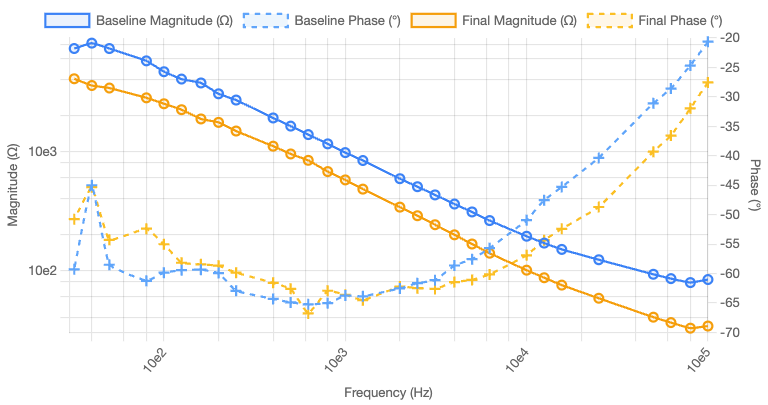
\includegraphics[width=\textwidth]{PBS_25_cropped.png}
        \caption{BioPal}
        \label{fig:25_pbs_biopal}
    \end{subfigure}
    \hfill
    \begin{subfigure}{0.48\textwidth}
        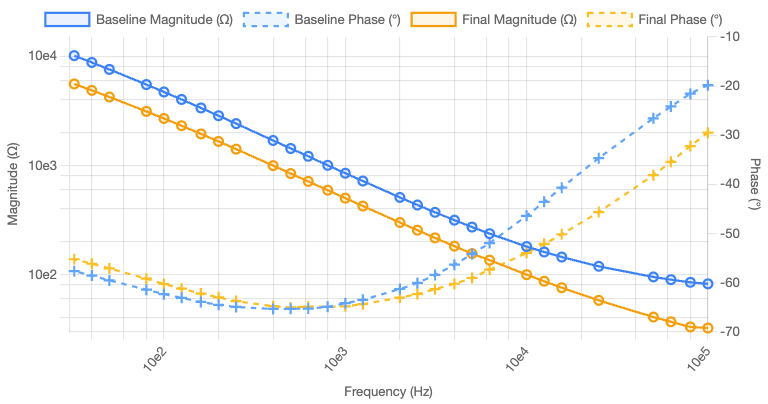
\includegraphics[width=\textwidth]{PalmSens_25.png}
        \caption{PalmSens4}
        \label{fig:25_pbs_palmsens}
    \end{subfigure}
    \caption{25\% Baseline vs 100\% Final PBS 1x Comparison}
    \label{fig:25_pbs_comparison}
\end{figure}
\begin{figure}[H]
    \centering
    \begin{subfigure}{0.48\textwidth}   
        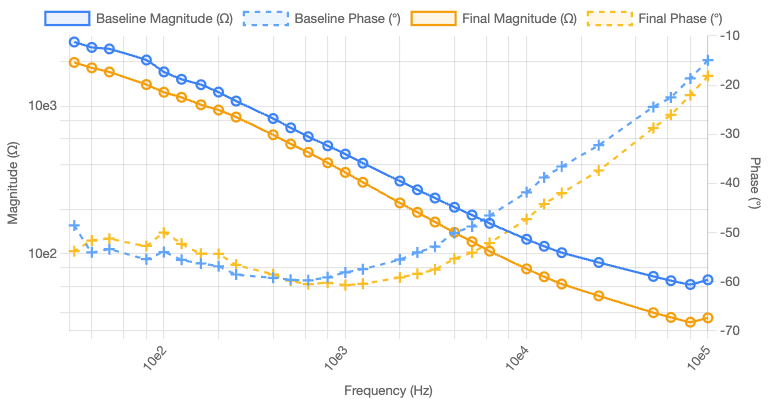
\includegraphics[width=\textwidth]{PBS_50_cropped.png}
        \caption{BioPal}
        \label{fig:50_pbs_biopal}
    \end{subfigure}
    \hfill
    \begin{subfigure}{0.48\textwidth}
        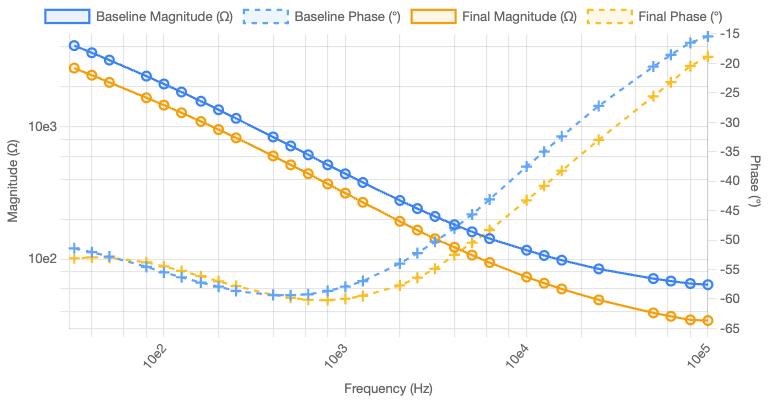
\includegraphics[width=\textwidth]{PalmSens_50.png}
        \caption{PalmSens4}
        \label{fig:50_pbs_palmsens}
    \end{subfigure}
    \caption{50\% Baseline vs 100\% Final PBS 1x Comparison}
    \label{fig:50_pbs_comparison}
\end{figure}

\begin{figure}[H]
    \centering
    \begin{subfigure}{0.48\textwidth}
        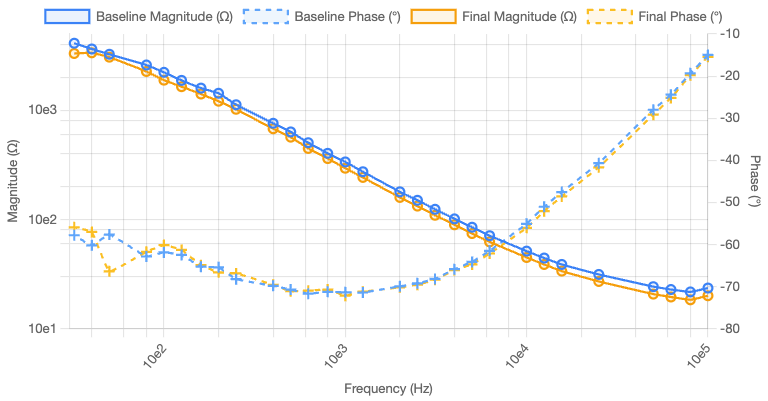
\includegraphics[width=\textwidth]{PBS_75_cropped.png}   
        \caption{BioPal}
        \label{fig:75_pbs_biopal}
    \end{subfigure}
    \hfill
    \begin{subfigure}{0.48\textwidth}
        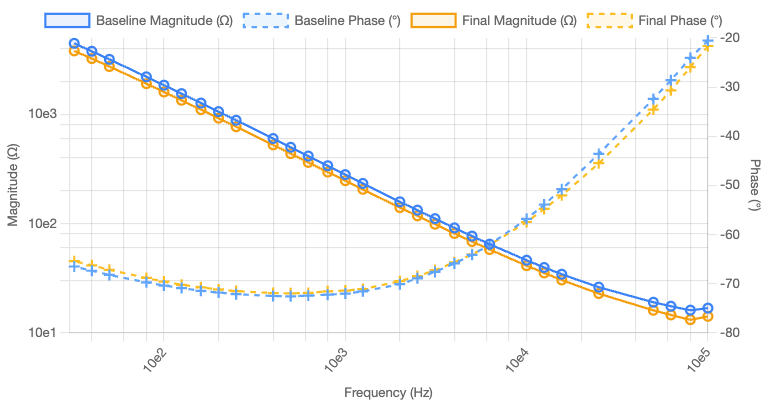
\includegraphics[width=\textwidth]{PalmSens_75.png}
        \caption{PalmSens4}
        \label{fig:75_pbs_palmsens}
    \end{subfigure}
    \caption{ 75\% Baseline vs 100\% Final PBS 1x Comparison}
    \label{fig:75_pbs_comparison}
\end{figure}


After validating the ability to distinguish bulk solution impedance changes, sensitivity to surface-based impedance changes needed to be confirmed. While testing with immobilised antibodies and actual protein antigens would provide the most direct validation, this was beyond the scope of this project due to laboratory safety restrictions, cost constraints, and limited time. Instead, BSA was used as a surface-binding protein to simulate antibody-antigen interactions. BSA is a common blocking protein that is readily absorbed by gold electrode surfaces, creating a protein layer that alters the interfacial impedance characteristics. This mimics the effect of antibody-antigen binding on the electrode surface.

The measurement methodology involved establishing a baseline impedance measurement in PBS 1x, removing the PBS and adding BSA solution to the electrode well, allowing 20 minutes for protein adsorption, flushing the electrode three times with fresh PBS 1x to remove unbound protein and thus maintaining the same solution characteristics, and finally performing a second impedance measurement.

Existing literature use BSA concentrations ranging from 1 mg/mL to 60 mg/mL for impedance based biosensor sensitivity validation \cite{maImpedancebasedIntegratedBiosensor2013}\cite{ebadiPolypyrrolebasedBovineSerum2025}. In this work, three concentrations were selected: 20 mg/mL, 50 mg/mL and 100 mg/mL.

Measurements were performed at each step using both the BioPal and the PalmSens4 for direct comparison. Figures \ref{fig:2g_bsa_comparison_final} - \ref{fig:10g_bsa_comparison_final} shows the impedance magnitude and phase measurements from both instruments before and after BSA binding, showing a clear difference between concentrations. Figures \ref{fig:2g_bsa_comparison} - \ref{fig:10g_bsa_comparison} show the relative change in magnitude across the frequency range. It was found that the largest impedance changes occurred in the frequency range from 160 Hz to 500 kHz. The average change in this range was used to give a qualitative result. The device gives the user a risk level of disease presence ranging from none to high based on the following thresholds:
\begin{table}[H]
\centering
\caption{Qualitative Risk Levels Based on Impedance Change}
\label{tab:risk_levels}
\begin{tabular}{lcccc}
\hline
\textbf{Risk Level} & \textbf{None} & \textbf{Low} & \textbf{Medium} & \textbf{High} \\
\hline
\textbf{Impedance Change} & \textless 5\% & 5\% - 15\% & 15\% - 25\% & \textgreater 25\% \\
\hline
\end{tabular}
\end{table}

% Now the same but for the baseline vs final of each concentration for biopal and palmsens next to eachother
\begin{figure}[H]
    \centering
    \begin{subfigure}{0.48\textwidth}
        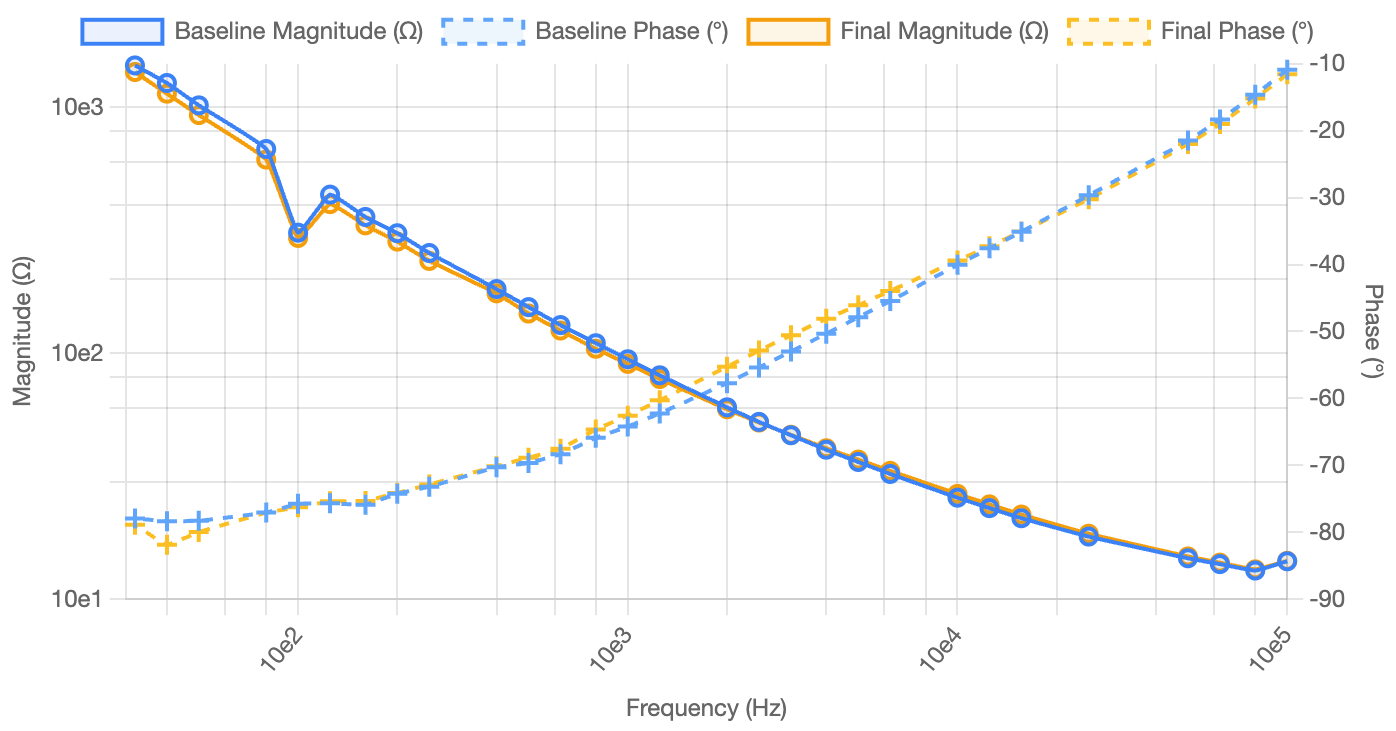
\includegraphics[width=\textwidth]{2g-100mL BioPal.png}
        \caption{BioPal: Baseline vs Post-BSA}
        \label{fig:2g_biopal}
    \end{subfigure}
    \hfill
    \begin{subfigure}{0.48\textwidth}
        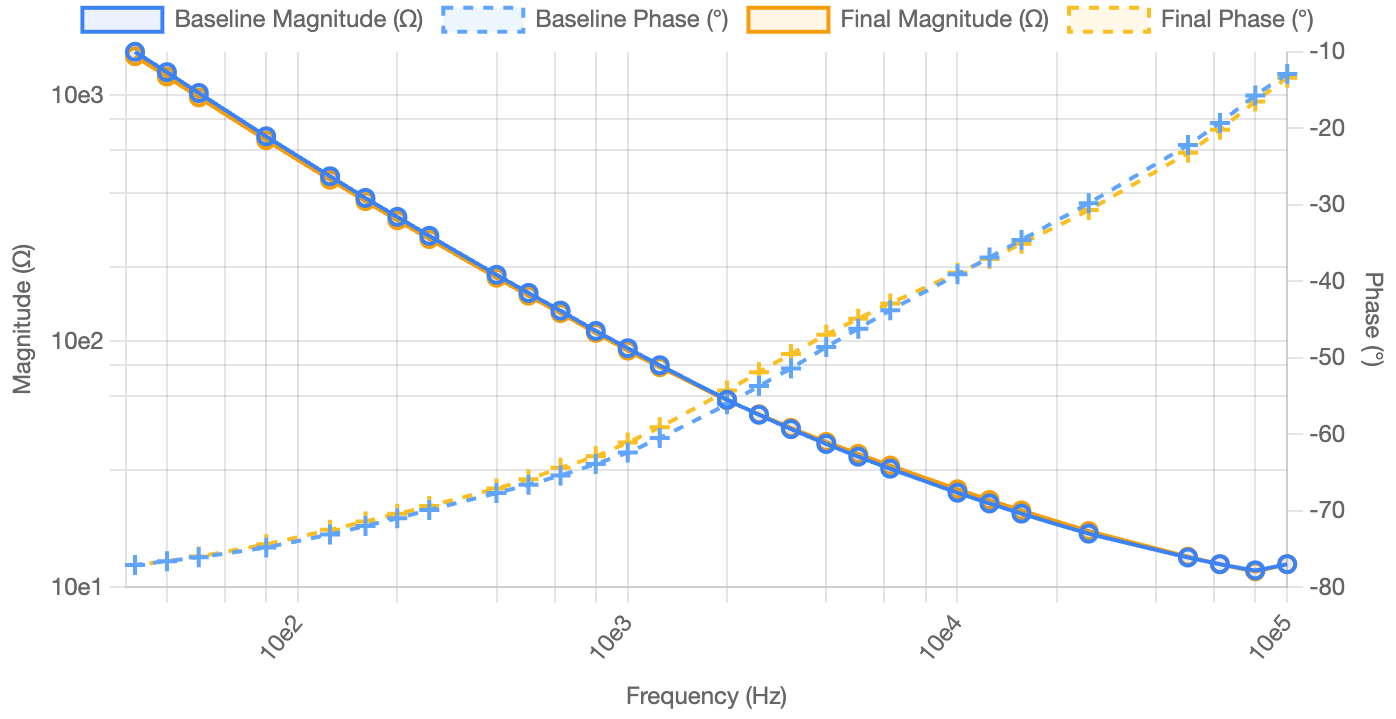
\includegraphics[width=\textwidth]{PalmSens2g.png}
        \caption{PalmSens4: Baseline vs Post-BSA}
        \label{fig:2g_palmsens}
    \end{subfigure}
    \caption{Baseline vs Final Frequency Response to 20mg/mL BSA Binding}
    \label{fig:2g_bsa_comparison_final}
\end{figure}

\begin{figure}[H]
    \centering
    \begin{subfigure}{0.48\textwidth}   
        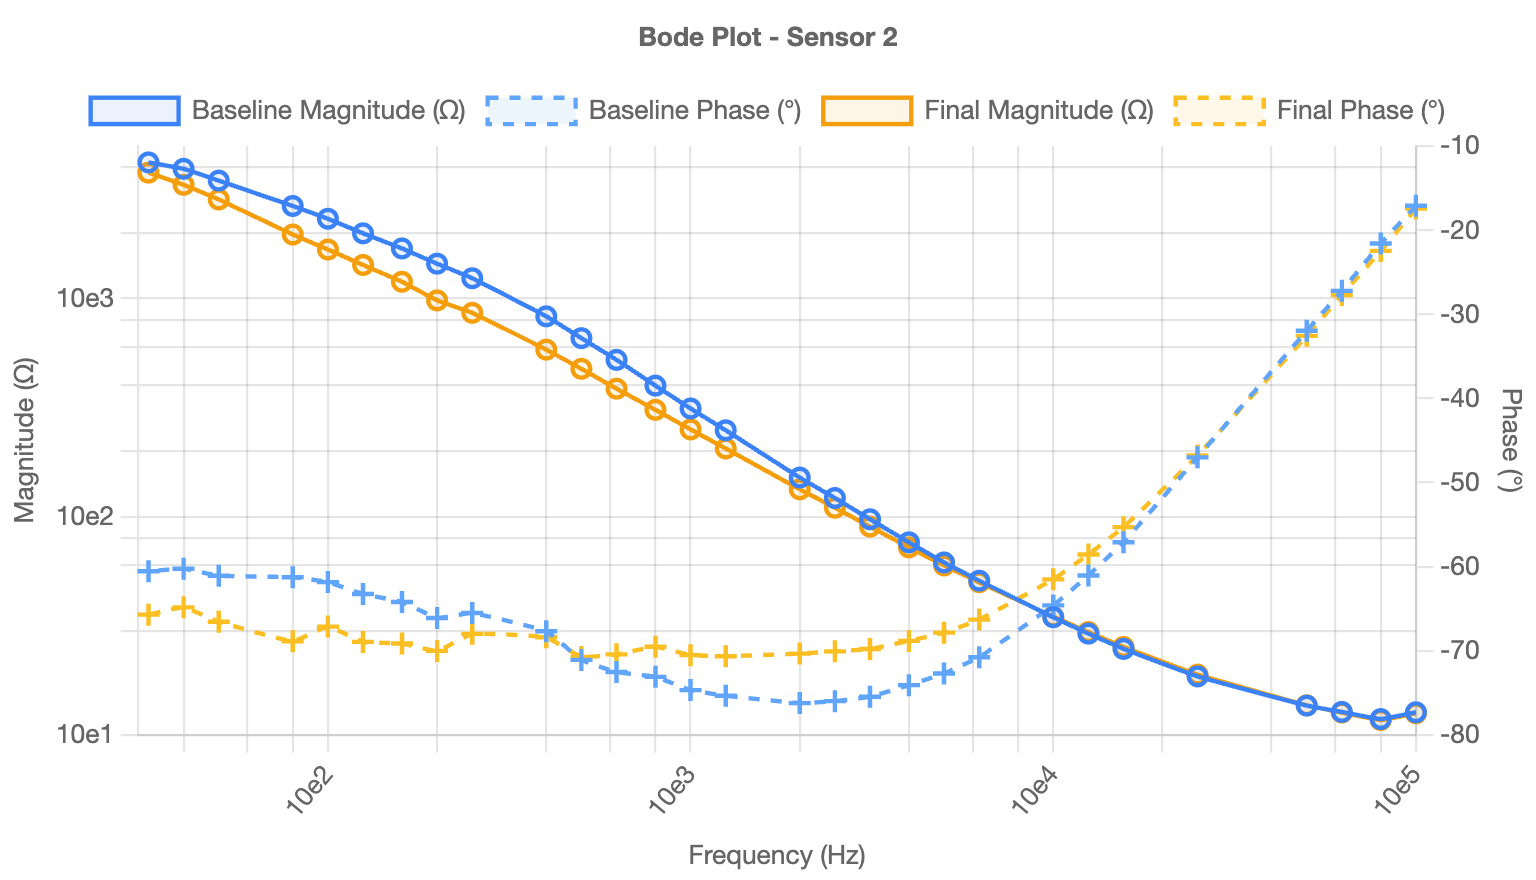
\includegraphics[width=\textwidth]{5g-100mL BioPal.png}
        \caption{BioPal: Baseline vs Post-BSA}
        \label{fig:5g_biopal}
    \end{subfigure}
    \hfill
    \begin{subfigure}{0.48\textwidth}
        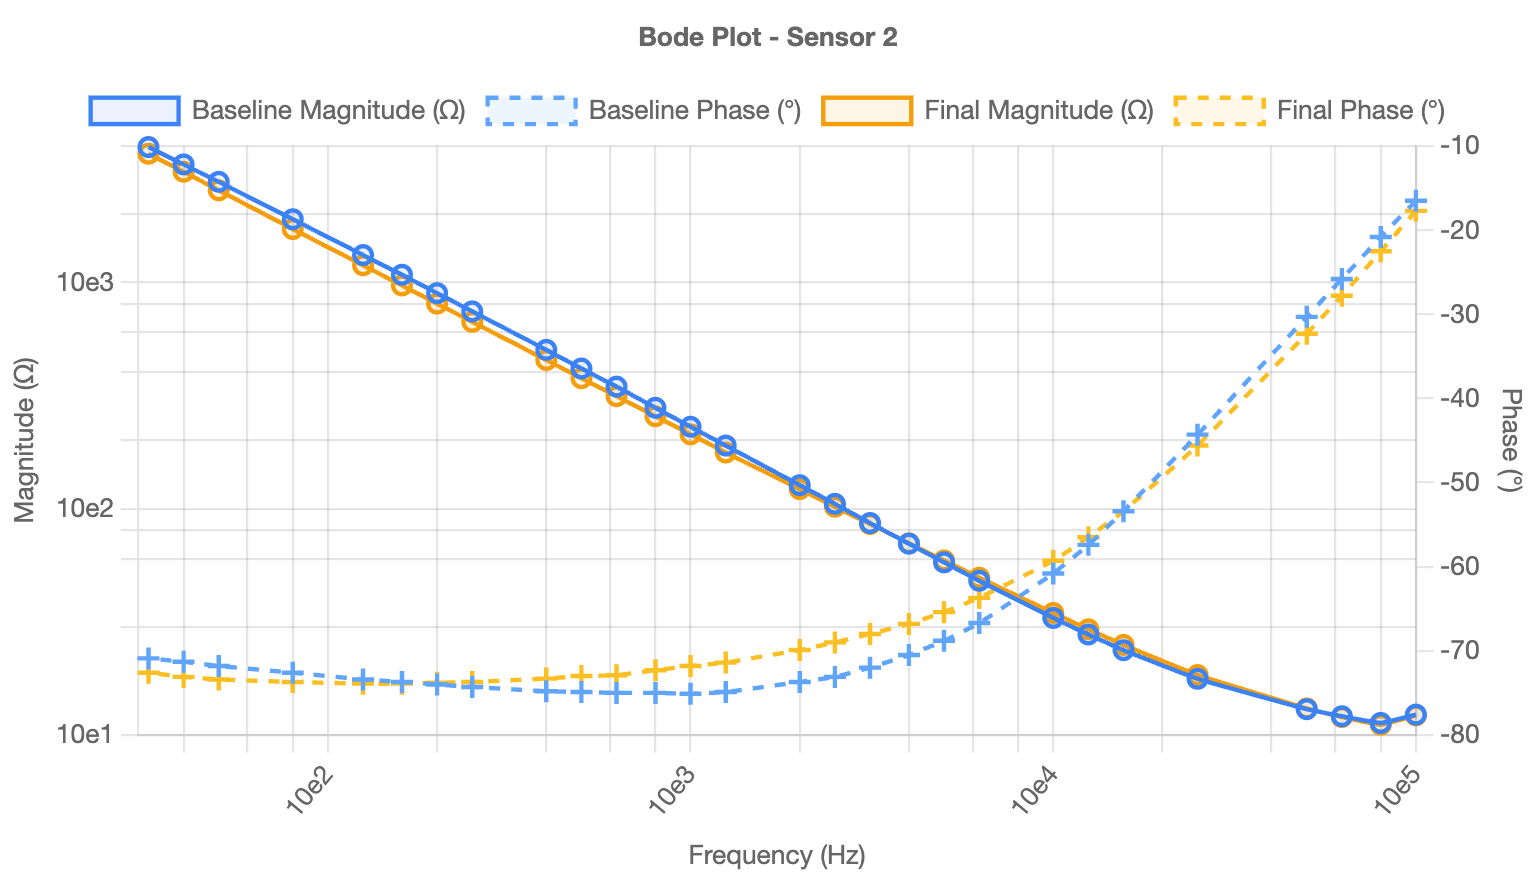
\includegraphics[width=\textwidth]{PalmSens5g.png}
        \caption{PalmSens4: Baseline vs Post-BSA}
        \label{fig:5g_palmsens}
    \end{subfigure}
    \caption{Baseline vs Final Frequency Response to 50mg/mL BSA Binding}
    \label{fig:5g_bsa_comparison_final}
\end{figure}

\begin{figure}[H]
    \centering
    \begin{subfigure}{0.48\textwidth}
        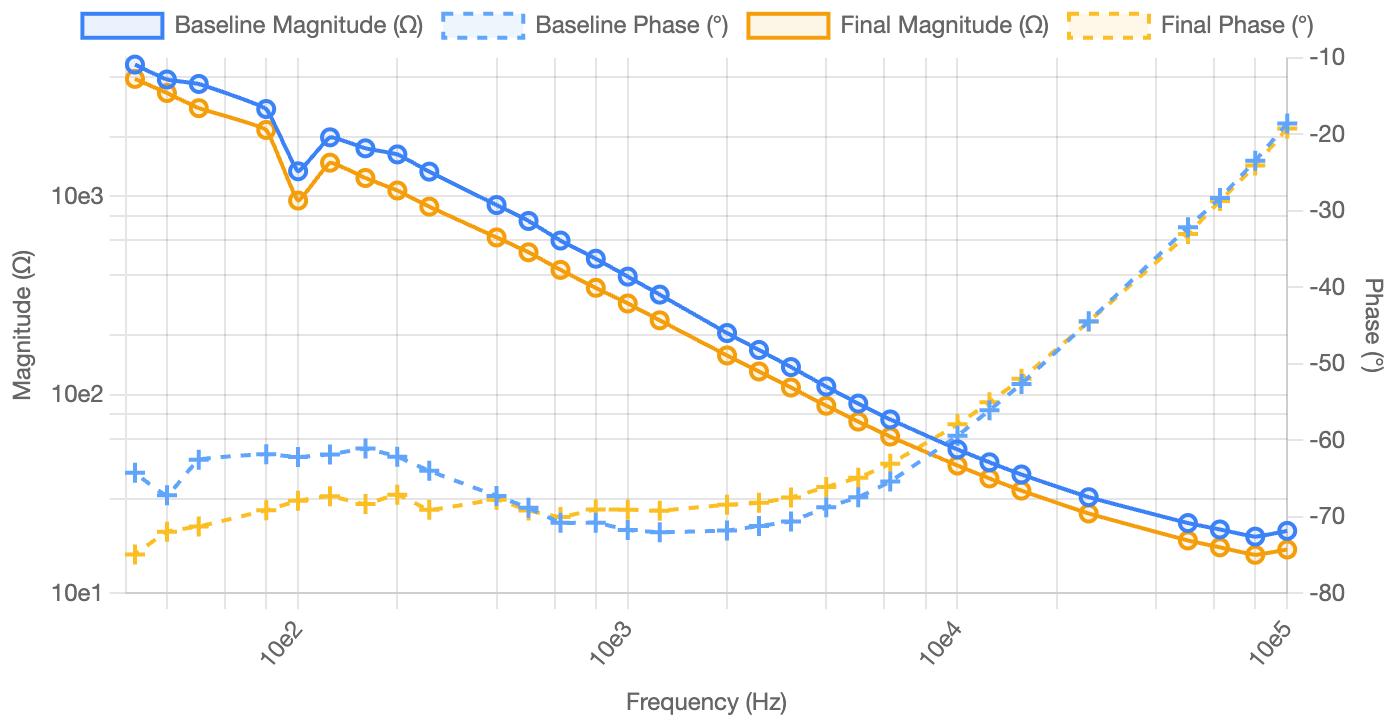
\includegraphics[width=\textwidth]{10g-100mL BioPal.png}   
        \caption{BioPal: Baseline vs Post-BSA}
        \label{fig:10g_biopal}
    \end{subfigure}
    \hfill
    \begin{subfigure}{0.48\textwidth}
        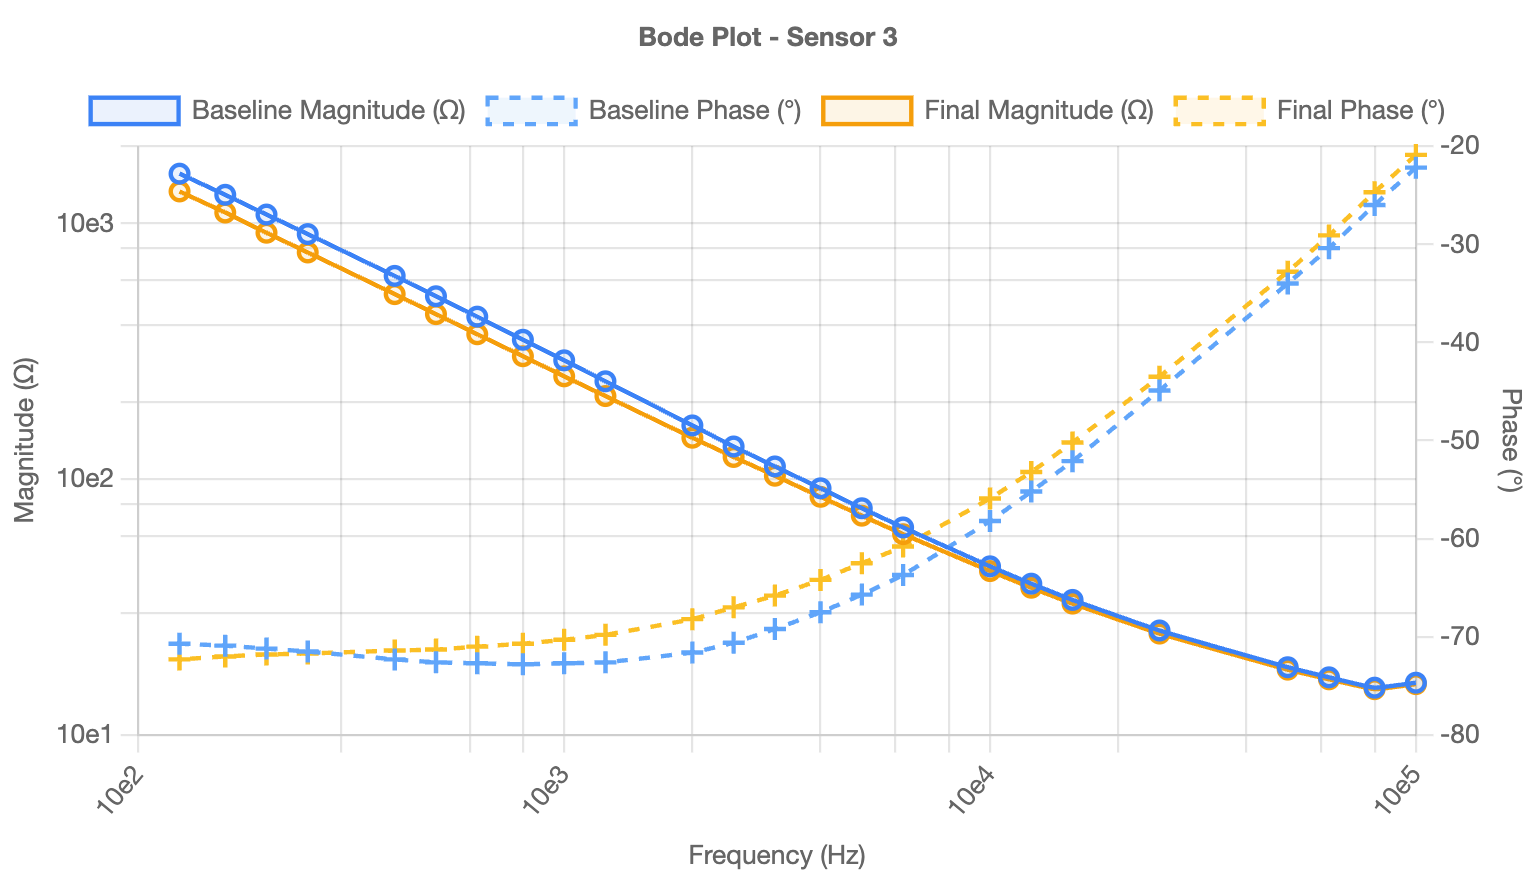
\includegraphics[width=\textwidth]{PalmSens10g.png}
        \caption{PalmSens4: Baseline vs Post-BSA}
        \label{fig:10g_palmsens}
    \end{subfigure}
    \caption{Baseline vs Final Frequency Response to 100mg/mL BSA Binding}
    \label{fig:10g_bsa_comparison_final}
\end{figure}

\begin{table}[H]
\centering
\caption{Average change in Impedance Magnitude due to BSA Binding (160 Hz - 500 Hz)}
\label{tab:risk_levels}
\begin{tabular}{lcccc}
\hline
\textbf{BSA Concentration} & \textbf{20 mg/mL} & \textbf{50 mg/mL} & \textbf{100 mg/mL} \\
\hline
\textbf{PalmSens4} & 2.8\% & 9.9\% & 15\% \\
\textbf{BioPal} & 6.7\% & 29.9\% & 31.7\% \\
\hline
\end{tabular}
\end{table}

% 3 seperate figures with subfigures (not minipages) showing the change in magnitude and phase for both instruments
\begin{figure}[H]
    \centering
    \begin{subfigure}{0.48\textwidth}
        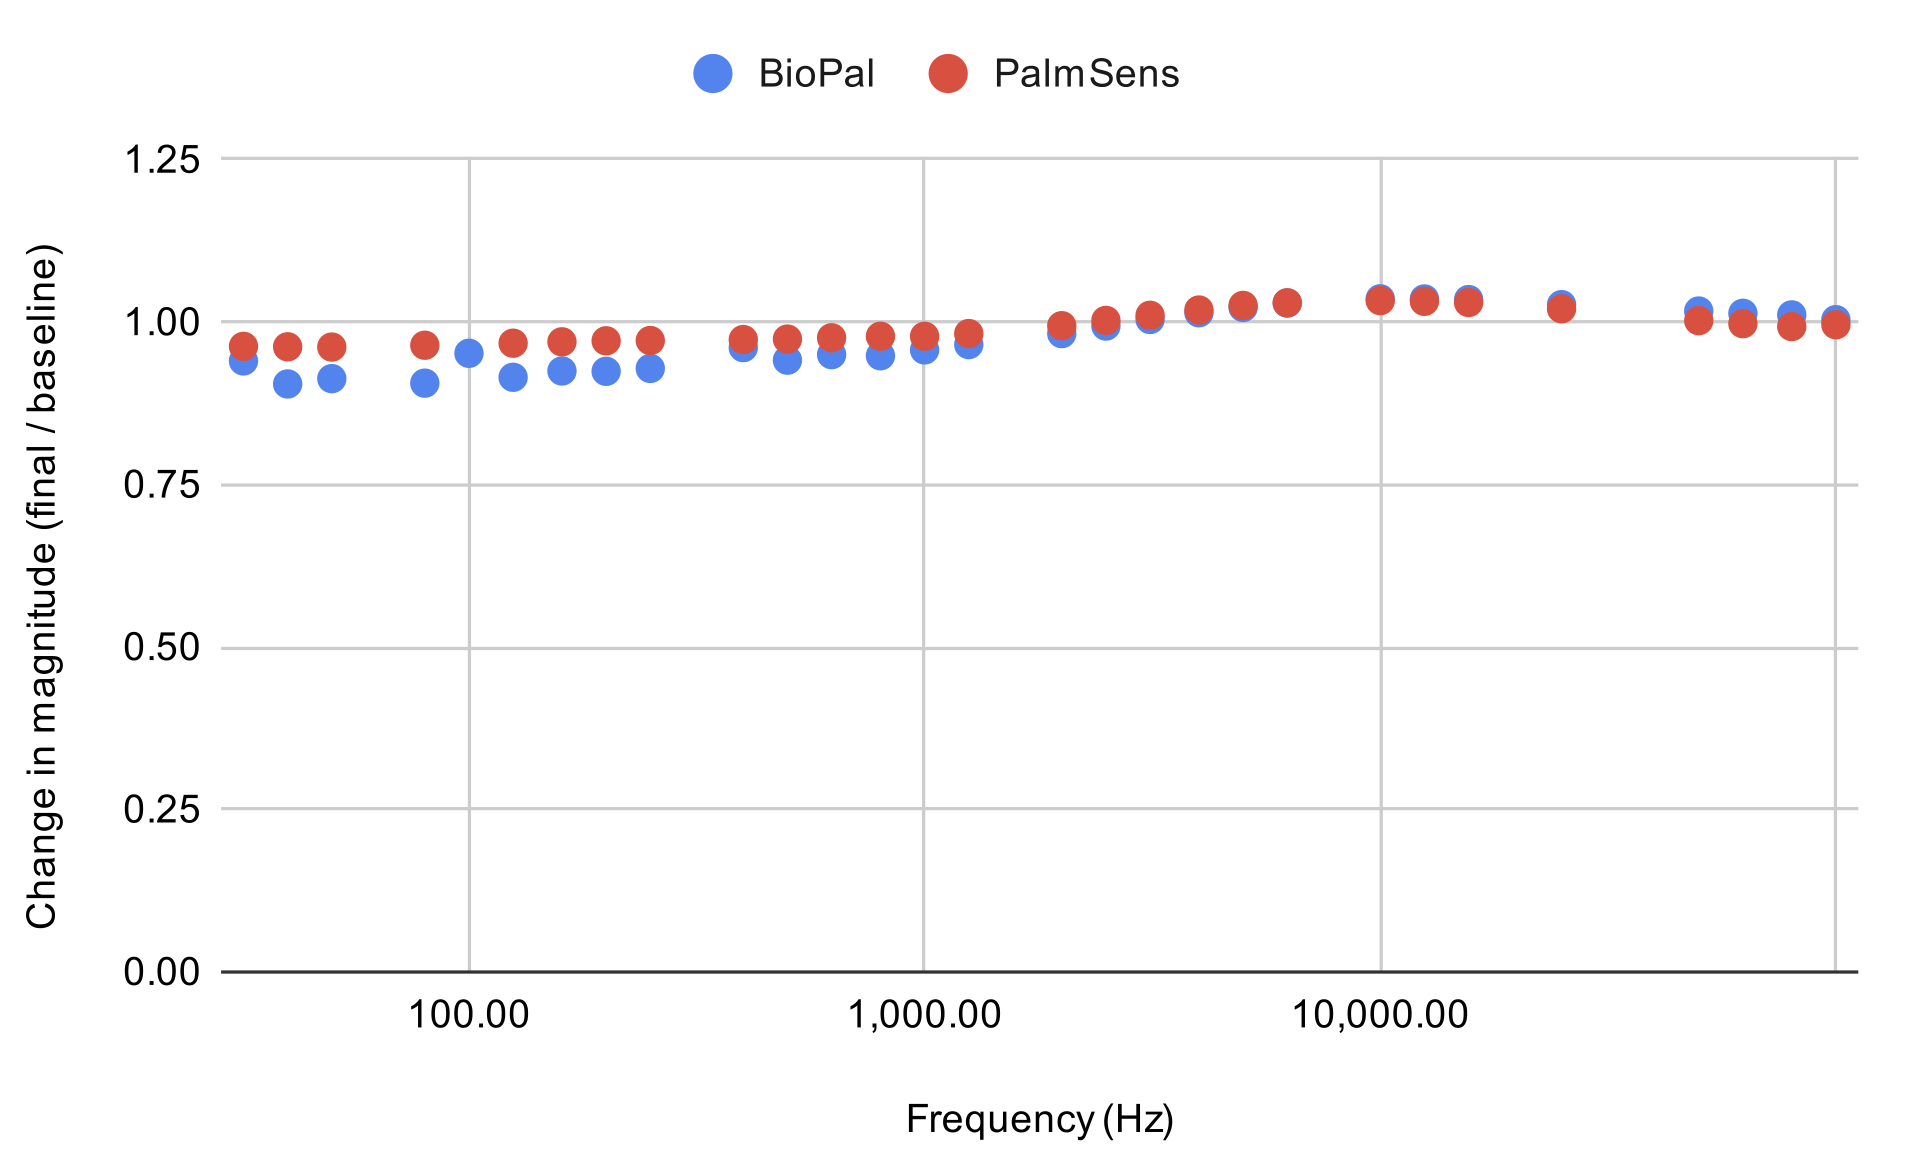
\includegraphics[width=\textwidth]{2g:100mL mag.png}
        \caption{Change in Impedance Magnitude}
        \label{fig:2g_mag}
    \end{subfigure}
    \hfill
    \begin{subfigure}{0.48\textwidth}
        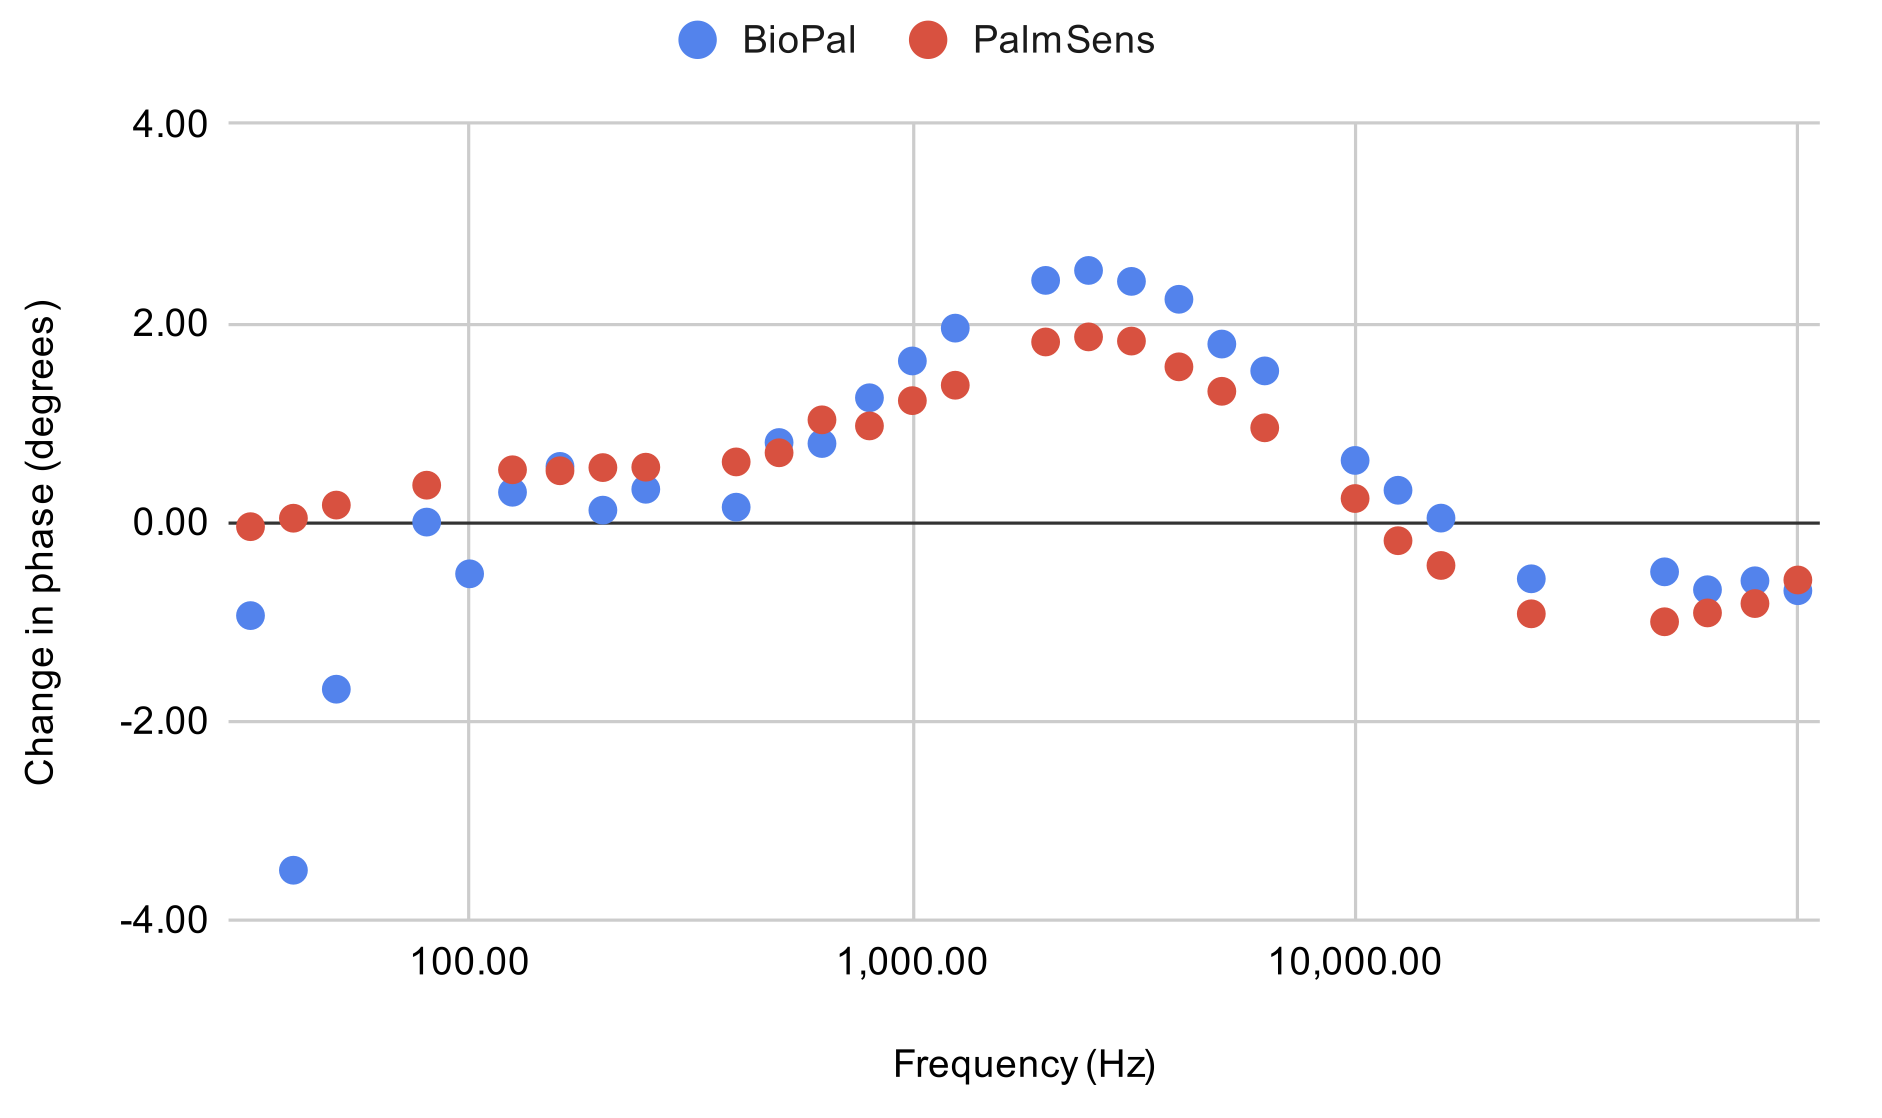
\includegraphics[width=\textwidth]{2g:100mL phase.png}
        \caption{Change in Impedance Phase}
        \label{fig:2g_phase}
    \end{subfigure}
    \caption{IDE Impedance Change with 20 mg/mL BSA Binding}
    \label{fig:2g_bsa_comparison}
\end{figure}

% 5g/100mL BSA
\begin{figure}[H]
    \centering
    \begin{subfigure}{0.48\textwidth}   
        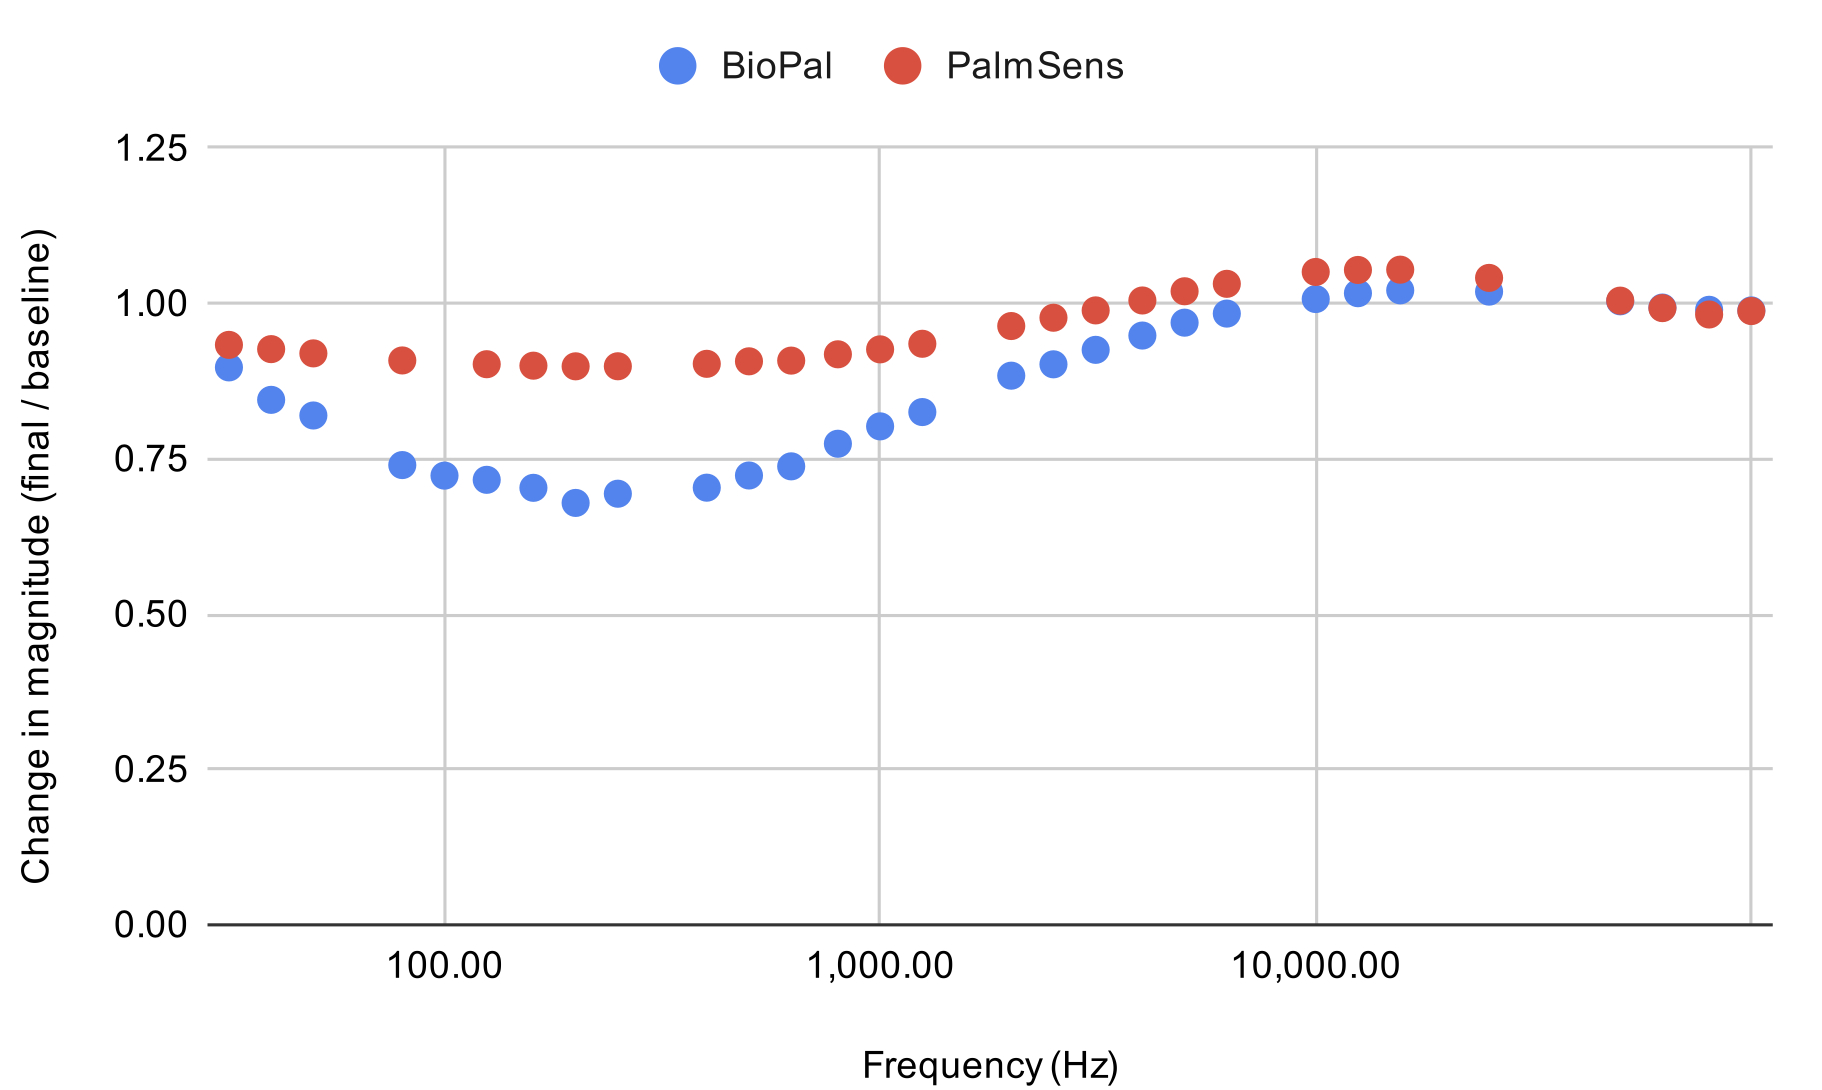
\includegraphics[width=\textwidth]{5g:100mL mag.png}
        \caption{Change in Impedance Magnitude}
        \label{fig:5g_mag}
    \end{subfigure}
    \hfill
    \begin{subfigure}{0.48\textwidth}
        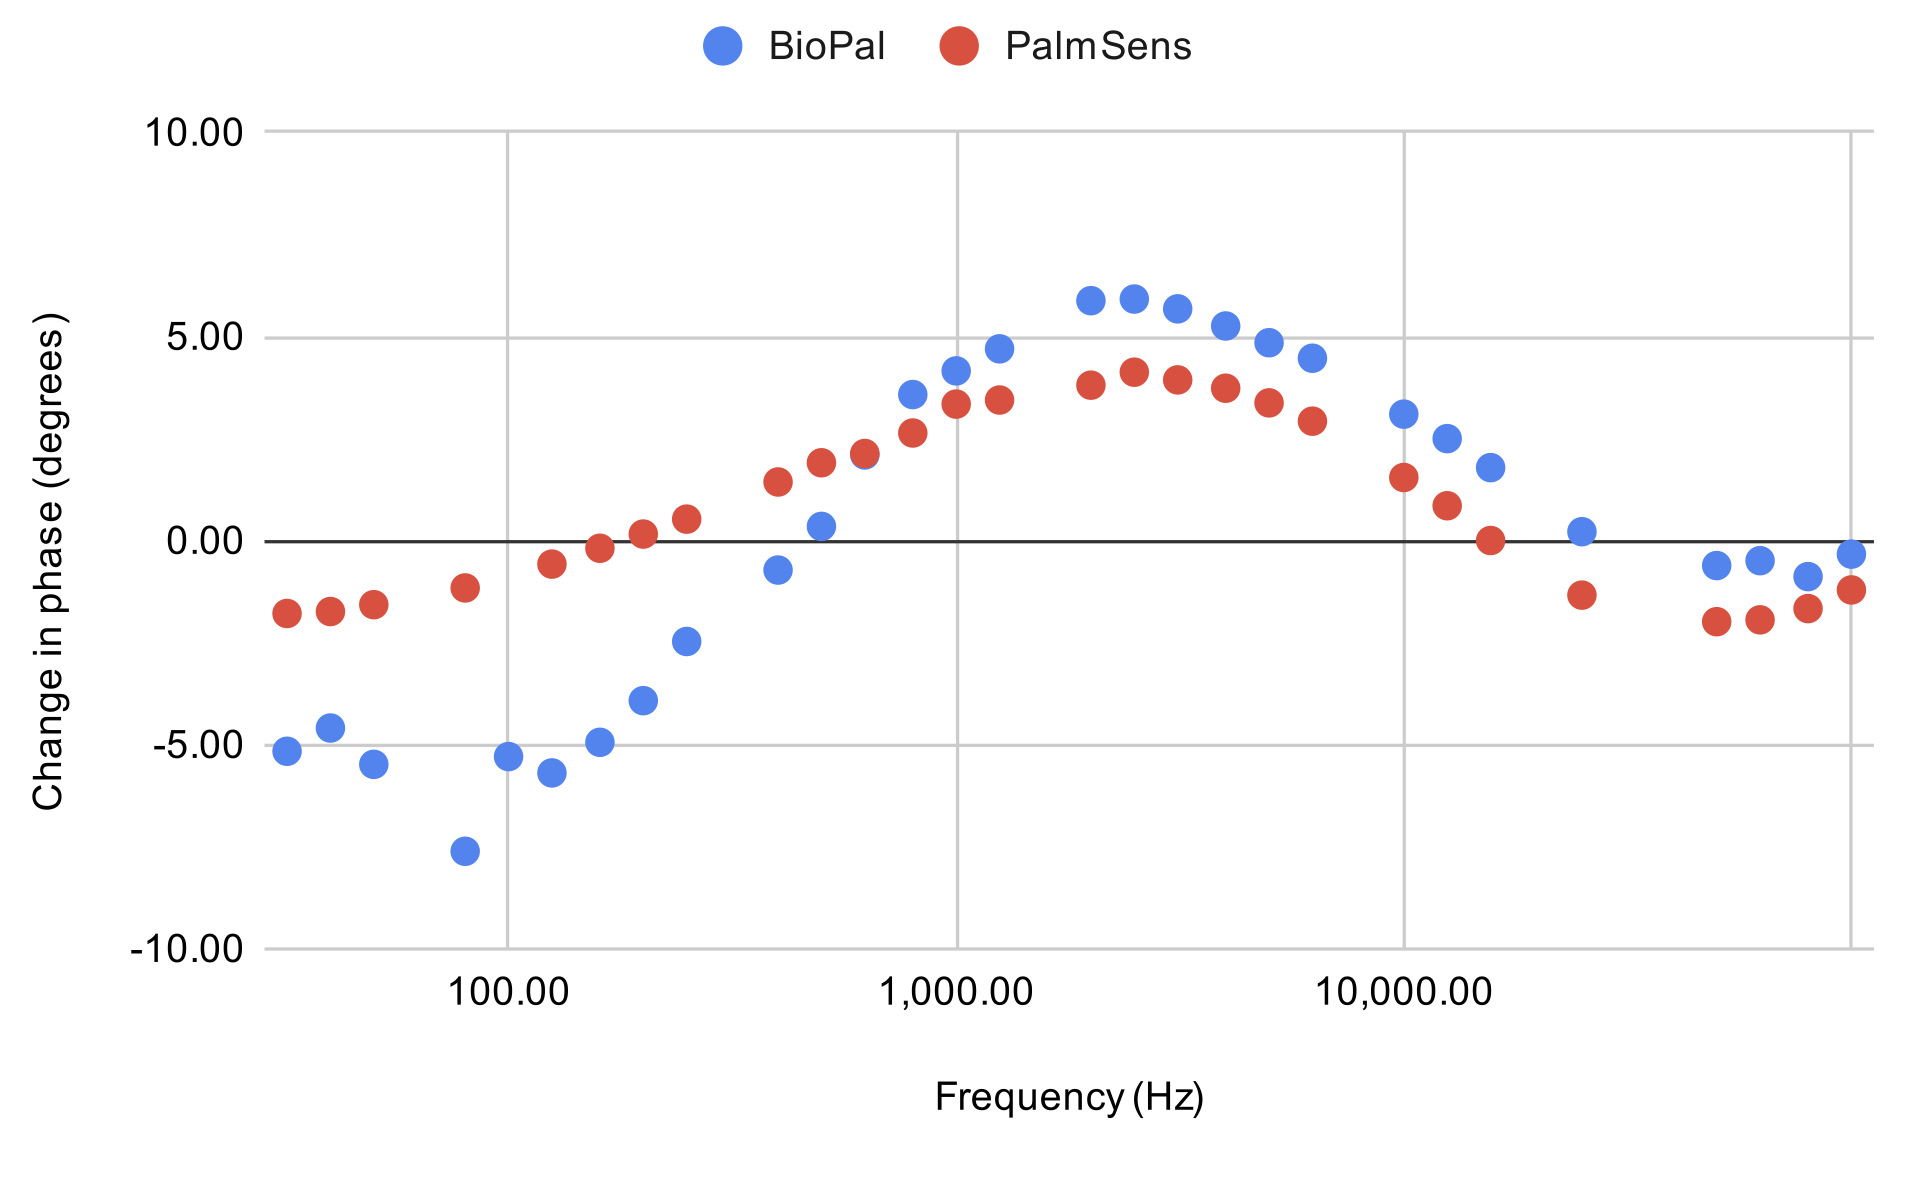
\includegraphics[width=\textwidth]{5g:100mL phase.png}
        \caption{Change in Impedance Phase}
        \label{fig:5g_phase}
    \end{subfigure}
    \caption{IDE Impedance Change with 50 mg/mL BSA Binding}
    \label{fig:5g_bsa_comparison}
\end{figure}

% 10g/100mL BSA
\begin{figure}[H]
    \centering
    \begin{subfigure}{0.48\textwidth}
        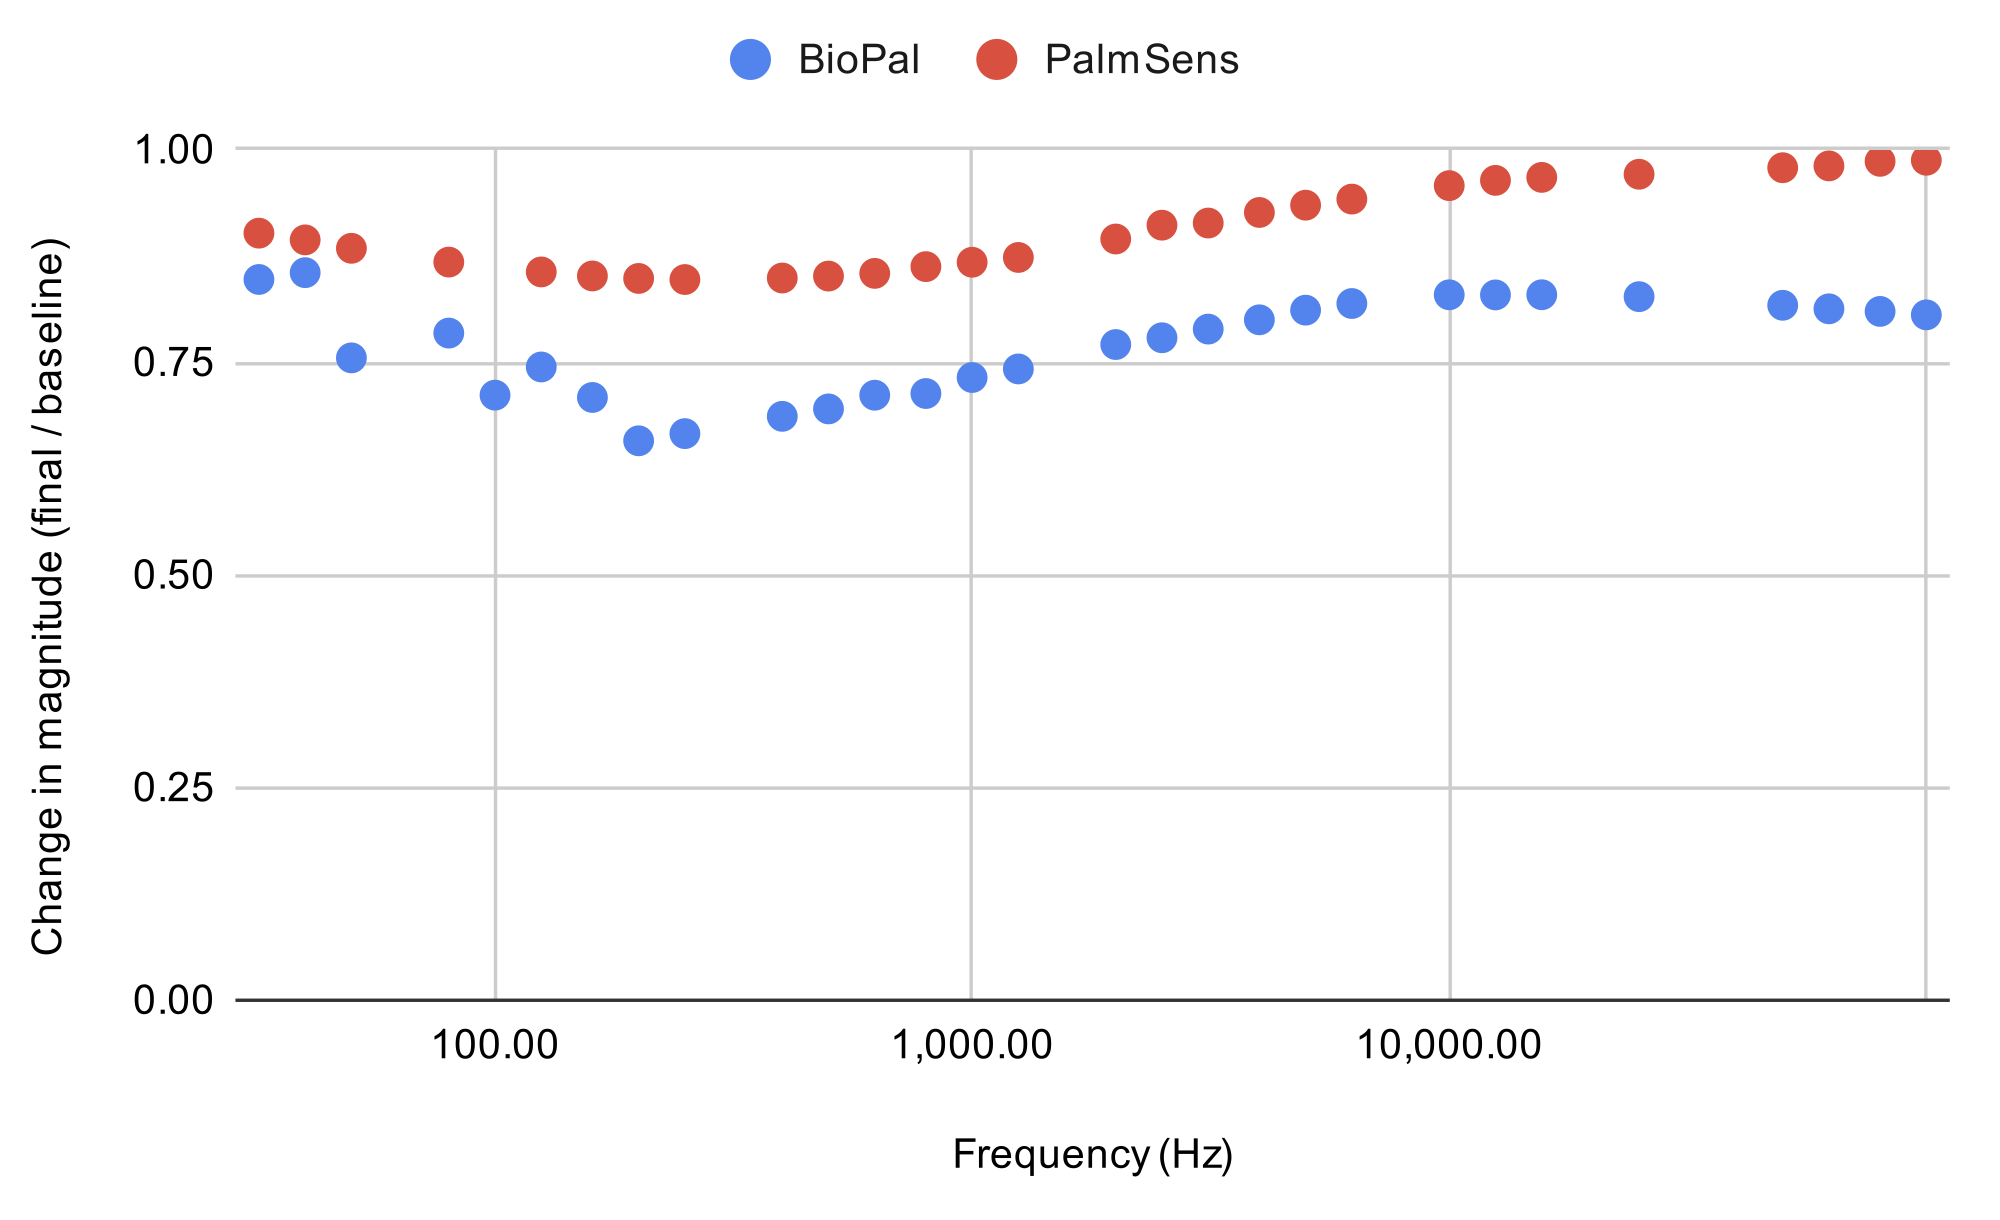
\includegraphics[width=\textwidth]{10g:100mL mag.png}   
        \caption{Change in Impedance Magnitude}
        \label{fig:10g_mag}
    \end{subfigure}
    \hfill
    \begin{subfigure}{0.48\textwidth}
        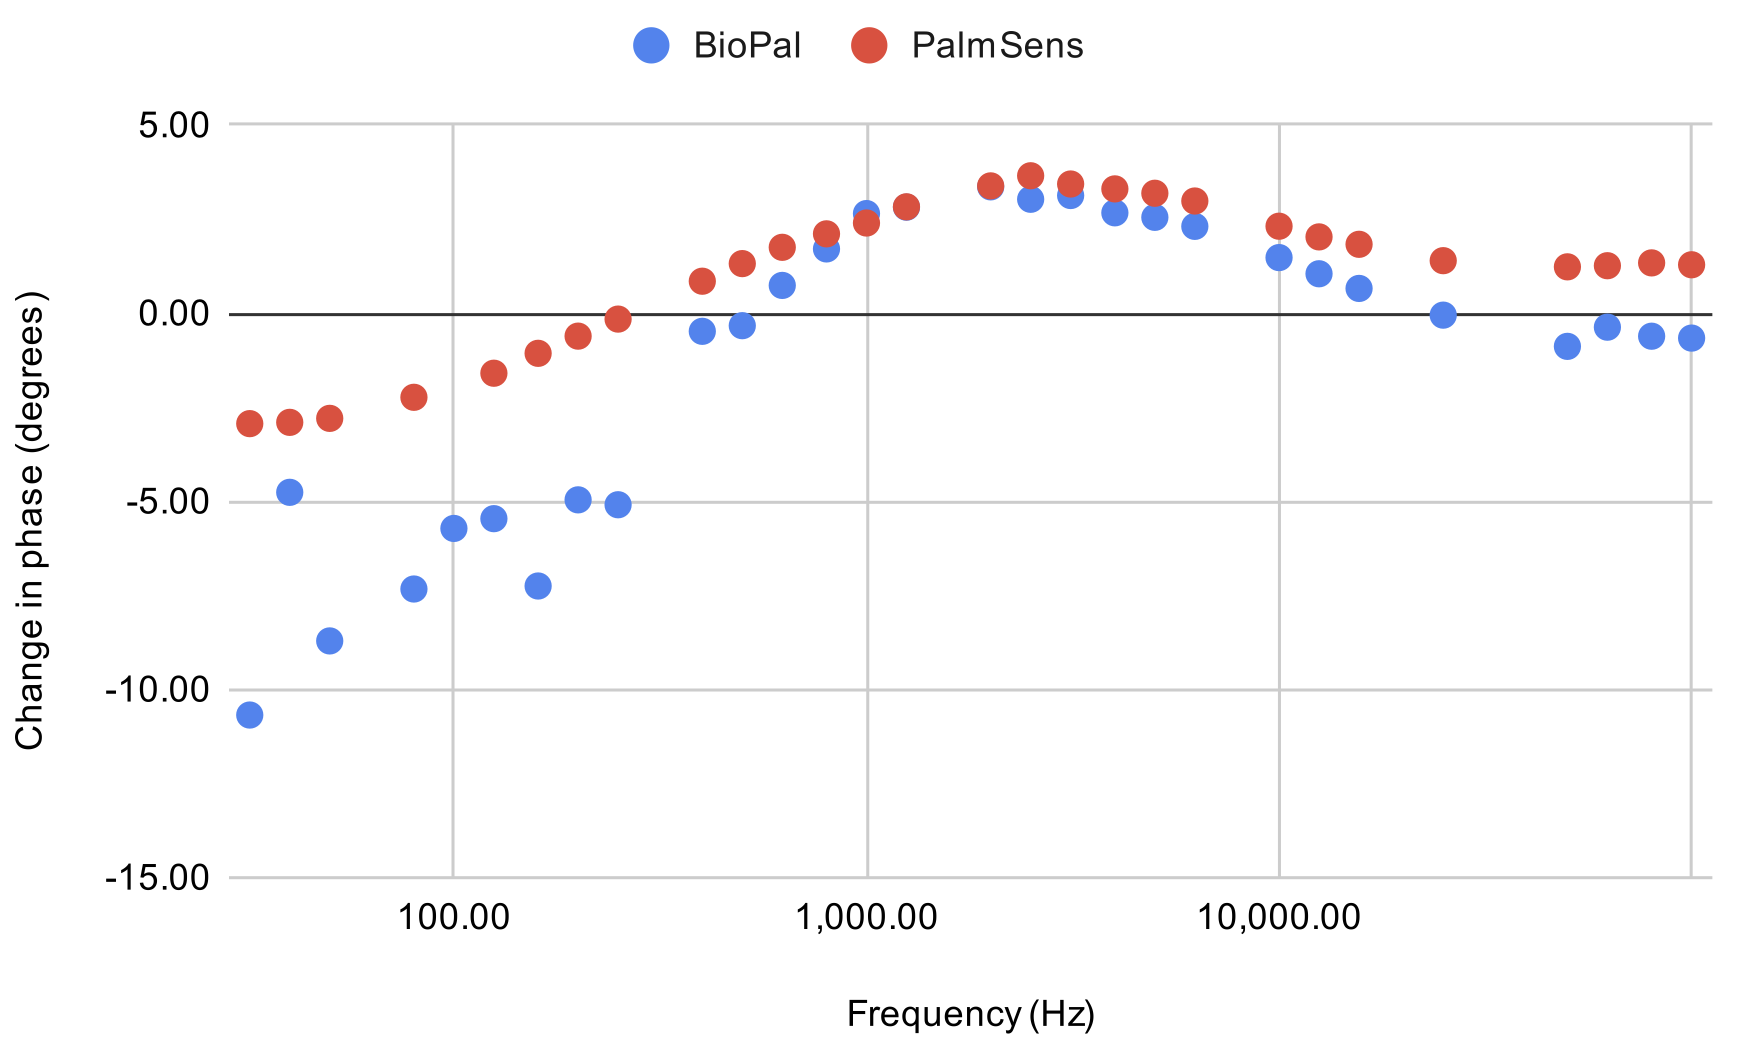
\includegraphics[width=\textwidth]{10g:100mL phase.png}
        \caption{Change in Impedance Phase}
        \label{fig:10g_phase}
    \end{subfigure}
    \caption{IDE Impedance Change with 100 mg/mL BSA Binding}
    \label{fig:10g_bsa_comparison}
\end{figure}

\section{Discussion of Validation Results}
The BioPal meets all requirements needed to meet the objectives set out in Chapter 1. All subsystems in the analogue frontend perform close to expectations and well within the requirements. The system is capable of performing impedance measurements with an average run to run standard deviation of 1.03\% from 125 Hz to 100 kHz. The majority of run to run variance occurs at lower frequencies due to the lack of anti-aliasing (as seen in Figure \ref{fig:std_dev} in Appendix \ref{appen:testing}). The multiplexed measurement system allows for up to 4 \acp{IDE} to be measured sequentially without human intervention and without impacting measurement accuracy.

PBS concentration measurements performed exceptionally well, with sub-3\% error margins across all tested concentrations (Table \ref{tab:pbs}), ensuring that different concentrations can be reliably distinguished. This validates the BioPal's impedance measurement capabilities and the core functionality of the combined system.  The lack of AA-filter had an impact at low frequencies, however this did not have an impact on final results due to being outside the range of interest for the tested \acp{IDE}. The frequency response closely tracked the PalmSens4 from 125 Hz to 100 kHz (Figures \ref{fig:25_pbs_comparison} - \ref{fig:75_pbs_comparison}), confirming that the calibration procedure successfully compensates for systematic errors in the analogue frontend.

Tests using BSA confirmed that the BioPal can clearly differentiate between different concentrations, albeit with larger error margins against the PalmSens than the PBS tests. Figures \ref{fig:2g_bsa_comparison} - \ref{fig:10g_bsa_comparison} show that the change in magnitude across the tested frequency range follows a similar pattern between the BioPal and PalmSens. However, the BioPal consistently detected larger changes than the PalmSens. This disparity likely results from the measurement sequence, with baselines first recorded with the BioPal then the PalmSens, while final measurements reversed this order (PalmSens then BioPal). The roughly 10 minute delay between BioPal and PalmSens measurements allowed time-dependent impedance reduction from PBS exposure \cite{moultonStudiesDoubleLayer2004}. Thus, the PalmSens baseline had more time to stabilize and the final had less, while the BioPal baseline had less time to stabilize and the final more time. This emphasises the importance of standardised measurement timing protocols for \ac{POC} deployment. Despite this, the BioPal was able to reliably distinguish between concentrations, demonstrating its suitability for biosensing applications. The risk level classification based on impedance change (Table \ref{tab:risk_levels}) functioned as intended, providing a straightforward interpretation of results for end-users.

Recommendations for future work as well as a summary of the completed project is discussed in the following chapter.

% The analogue frontend performed according to specifications across most of the target range. However, the failed LTC1069 AA filter caused aliasing artefacts below 32 Hz, limiting accurate measurements to higher frequencies. This proved acceptable for the tested IDEs (160 Hz to 500 kHz), but replacement would be essential for biosensors requiring lower frequency measurements. The dual-microcontroller architecture effectively balanced measurement precision (STM32) with system control and user interface requirements (ESP32).
\label{chap:testing_and_validation}